%% Sports Medicine - Open — Original Research Article — FIRST DRAFT (29 Oct 2026)
%% Reference style: Vancouver (numbered, square brackets) — unsrt.bst with natbib [numbers]
%% Builds on the accepted SMO manuscript's LaTeX setup (RAE paper, SMOA-D-26-00548).

\documentclass[12pt,a4paper]{article}

\usepackage[utf8]{inputenc}
\usepackage[T1]{fontenc}
\usepackage{times}
\usepackage[margin=2.5cm]{geometry}
\usepackage{setspace}
\doublespacing

\usepackage{graphicx}
\graphicspath{{../figures/}}
\usepackage{float}
\usepackage{placeins}
\usepackage{amsmath,amssymb}
\usepackage{booktabs}
\usepackage{makecell}
\usepackage{enumitem}
\usepackage[colorlinks=true,linkcolor=blue,citecolor=blue,urlcolor=blue]{hyperref}
\usepackage[numbers,sort&compress]{natbib}
\usepackage{lineno}
\linenumbers

\begin{document}

% ── Title page ──────────────────────────────────────────────

\begin{titlepage}
\vspace*{2cm}

{\noindent\LARGE\bfseries Stagnation before exit: within-athlete performance progression, relative age, and retention in youth track and field --- a population register study\par}

\vspace{1.5cm}

{\noindent\large
Atle G.\ Guttormsen$^{1,*}$ \\
\href{https://orcid.org/0000-0003-0188-8462}{ORCID: 0000-0003-0188-8462}
}

\vspace{0.8cm}

{\noindent
$^1$School of Economics and Business, Norwegian University of Life Sciences (NMBU), Ås, Norway
}

\vspace{0.8cm}

{\noindent
$^*$Corresponding author:\\
Atle G.\ Guttormsen\\
School of Economics and Business\\
Norwegian University of Life Sciences (NMBU)\\
P.O.\ Box 5003, 1432 Ås, Norway\\
E-mail: atle.guttormsen@nmbu.no
}

\vspace{1.5cm}

{\noindent\textbf{Word count:} $\sim$4\,500 (main text, excluding abstract, references, tables, and figure legends)}

\end{titlepage}

% ── Abstract ────────────────────────────────────────────────

\newpage
\section*{Abstract}

\noindent\textbf{Background.} Athletes withdraw from organised youth sport through a gradual behavioural process: competition volume declines years before formal exit. Whether the athlete's own \emph{performance development} carries additional prospective information --- whether stagnation precedes exit --- has not been tested in population data, and a companion registry study proposed exactly this test of its mastery-experience interpretation: that visible personal progress retains athletes, particularly those born late in the selection year.

\noindent\textbf{Methods.} Using the Norwegian Athletics Federation's complete competition registry, all athletes born 1998--2005 with an approved result at age 13--14 and at 15--16 formed a landmark cohort (n = 3\,808; 53\,\% female; 648 [17.0\,\%] later active as seniors, age $\geq$20). Progression was the change in age-graded performance points (mean of the three best scores in the athlete's main event group) from ages 13--14 to 15--16. Logistic regression estimated the association with senior activity beyond sex, cohort, performance level, competition volume in both windows, and the number of scored results; discrimination was assessed with repeated cross-validation. Pre-specified tests examined whether the association was stronger among relatively younger athletes (birth-quarter interaction) and how progression compared with level. The analysis plan was committed to version control before estimation; the study was not externally preregistered.

\noindent\textbf{Results.} Progression predicted senior activity with OR = 2.02 per SD (95\,\% CI 1.73--2.37), adding modestly to discrimination (cross-validated AUC 0.855 to 0.864). The association replicated in both birth cohorts (OR 2.00 and 2.03), was unchanged under club clustering and COVID-19-window exclusions, and a within-baseline specification check was null (OR 1.00). The E-value was 2.84. Dropouts' points fell 7 below their own level in the penultimate season and 48 in the final season, mirroring the decline in competition volume. The birth-quarter interaction was null (OR 0.95, 95\,\% CI 0.85--1.07): progression predicted retention in both relatively older (OR 2.19) and relatively younger athletes (OR 1.89). Given volume, progression and level discriminated equally.

\noindent\textbf{Conclusions.} Stagnation precedes exit from youth track and field: within-athlete performance progression predicts senior retention as strongly as competition volume predicts it, independently of both volume and level. The association is general rather than specific to relatively younger athletes, supporting a broad progression--retention link but not the relative-age-specific mastery prediction. Registry-based athlete monitoring can read declining progression, alongside declining participation, as an early signal of disengagement --- while causal interpretation must await designs that can separate commitment, injury, and development.

\vspace{0.5em}
\noindent\textbf{Keywords:} youth sport; dropout; athlete retention; performance development; relative age effect; registry study; track and field

% ── Key points ──────────────────────────────────────────────

\section*{Key Points}
\begin{itemize}[leftmargin=1.2em]
  \item In a national competition registry following 3\,808 athletes from ages 13--16 into adulthood, within-athlete performance progression predicted senior retention with an odds ratio of 2.0 per SD --- as strong as the best known behavioural predictor, competition volume --- independently of volume, level, and the number of results.
  \item Future dropouts stagnated before they left: their age-graded performance fell 7 points below their own earlier level in the penultimate season and 48 points in the final season, in parallel with their withdrawal from competition.
  \item The progression--retention association was equally strong among early-born and late-born athletes, supporting a general link between visible progress and continued participation but not the relative-age-specific mastery mechanism proposed in earlier registry work.
\end{itemize}

\newpage

% ════════════════════════════════════════════════════════════
\section{Background}

Withdrawal from organised youth sport is extensive, and its documented predictors are mostly motivational and structural rather than performance-related: loss of enjoyment is the dominant prospective predictor \cite{vanyperen2021,crane2015}, costs and social background shape who leaves \cite{espedalen2022}, a large share of turnover in talent systems is the system's own de-selection \cite{gullichbarth2026,filo2026}, and markers of early specialisation have failed to predict actual dropout when tested directly \cite{larson2019}. Performance itself has an ambiguous role. Junior performance predicts senior performance poorly \cite{kearney2018,gullich2022sm,gullich2025}, and in the most direct registry test to date, performance level at a single early milestone added little to a simple behavioural signal --- how often the athlete competed \cite{guttormsen2026dropout}.

Three analyses of the same national registry motivate the present study. First, a longitudinal study of performance development showed that cross-sectional youth rankings are dominated by compositional turnover --- the best performers at one age are largely different people from the best at the next --- without studying who exits or why \cite{guttormsen2026development}. Second, a 14-year cohort study showed that exit is behaviourally foreshadowed: future dropouts' competition volume fell 12\,\% below their own earlier level two seasons before exit and 23\,\% one season before, and volume at ages 13--14 predicted senior retention better than age-graded performance level did \cite{guttormsen2026dropout}. Third, a population-wide analysis of relative age found the birth-quarter skew fully established at age 10 and stable to age 25, and proposed a mastery-experience interpretation: in a sport where every result is an objective personal measure, visible personal progress may retain athletes independently of rank --- and it stated the direct test, namely ``whether within-athlete performance \emph{progression}, rather than performance level, predicts retention among relatively younger athletes specifically'' \cite{guttormsen2026rae}. No population study has linked objective within-athlete performance trajectories to subsequent dropout, in this or, to our knowledge, any comparable sport system.

This study performs that test. Among athletes still competing at ages 15--16, we ask three pre-specified questions. \textbf{H1:} does within-athlete progression from ages 13--14 to 15--16 predict being active as a senior, beyond sex, performance level, competition volume (level and change), and the number of results the progression measure is computed from? \textbf{H2:} is the association stronger among relatively younger athletes, as the mastery-experience interpretation predicts? \textbf{H3:} does progression, rather than level, carry the performance-related signal? Interpretation rules were fixed in advance. In particular, a null or weak H1 would \emph{not} falsify the mastery account, because the registry cannot distinguish disengagement from transfer to another sport in which the athlete is also progressing; a positive H1 with a null H2 would support a general progression--retention link but not the relative-age-specific mechanism. The analysis plan, including hypotheses, estimands, model specifications, and these interpretation rules, was written and committed to version control before any exposure--outcome model was estimated; the study was not preregistered on an external registry.

% ════════════════════════════════════════════════════════════
\section{Methods}

\subsection{Data source and design}

The Norwegian Athletics Federation's results database records every sanctioned competition result in Norway, plus Norwegian athletes' results abroad, and is electronically complete from 2011. We used a frozen extract of 29 October 2026 (results dated on or before that day). The design is a retrospective landmark cohort reported according to STROBE \cite{vonelm2007}. Age is calendar-year age (competition year minus birth year), the basis of age classes in Norwegian athletics.

\subsection{Sample}

All athletes born 1998--2006 entered the extraction (n = 32\,447); 12\,938 had at least one approved result at age 13--14. The landmark condition --- at least one approved result at ages 13--14 \emph{and} at 15--16 --- was met by 4\,910 athletes, of whom 4\,909 had known sex. Prediction is made from the end of the age-16 season, so the conditioning on early-adolescent survival is explicit rather than hidden \cite{anderson1983}. We excluded 734 athletes without scorable age-graded results in their main event group in both windows (among them athletes who left their original event group entirely; a sensitivity analysis recovers them) and 3 athletes in sex $\times$ event-group cells with fewer than 20 athletes. The primary sample comprises 3\,808 athletes born 1998--2005, all with at least nine years of follow-up; cohorts born 2006 were retained only for a secondary outcome. Of the primary sample, 648 (17.0\,\%) met the senior-activity outcome. Forty-three athletes lacked an exact birth date and were excluded from the birth-quarter analysis only (H2 n = 3\,781).

\subsection{Exposure: within-athlete progression}

Each result at ages 13--16 was converted to age-graded points with the Norwegian federation's Tyrving tables, which score a performance against age-, sex-, and event-specific reference standards; we used a workbook-exact implementation validated cell-by-cell against the official tables in earlier work on this registry \cite{guttormsen2026dropout,nfif2014}. Because the tables are age-calibrated, a constant score over time means developing exactly as the age norms expect; a falling score means falling behind them.

The athlete's \emph{main event group} is the event category (sprints, jumps, middle distance, throws) with most results at ages 13--14. Progression $\Delta$ is the mean of the three best scores in the main event group at ages 15--16 minus the same quantity at 13--14. We used the mean of the three best rather than the single best because a maximum rises mechanically with the number of attempts, which would entangle progression with competition volume; the number of scored results in each window ($k_{13}$, $k_{15}$) additionally enters all models as covariates. Manual-timed results were excluded from scoring. Progression and level were standardised within sex $\times$ main event group over the primary sample, since the tables are unequally demanding across event groups; volumes were standardised to the primary-sample SD.

\subsection{Outcome}

The primary outcome, identical to the companion cohort study \cite{guttormsen2026dropout}, is \emph{active senior}: at least two approved results in the same calendar year at age 20 or older, with follow-up to the extract date. Secondary outcomes were at least one result at age $\geq$20; at least one result at age $\geq$18 (allowing the 2006 cohort); and at least two results in a year at ages 20--21 (a fixed window equalising opportunity across cohorts).

\subsection{Covariates}

Sex; birth cohort; performance level (mean of three best scores at 13--14, standardised); competition volume as distinct competition days at 13--14 and at 15--16, so that volume enters as level \emph{and} change, mirroring the companion study; $k_{13}$ and $k_{15}$; region (modal competition district at 13--14); and baseline club (modal club at 13--14) with a club-size proxy (log of the number of study athletes in the club). Birth quarter (Q1--Q4) was computed from exact birth dates.

\subsection{Statistical analysis}

Nested logistic models were fitted on the primary sample: M0 (sex, cohort, region, club size), M1 (M0 + level + volume 13--14 + volume 15--16 + $k_{13}$ + $k_{15}$), and M2 (M1 + $\Delta$). H1 is the OR per SD of $\Delta$ in M2 and the gain in discrimination from M1 to M2, estimated by stratified 5-fold cross-validation repeated 20 times (percentile intervals over repetitions), with calibration slope and Brier score from out-of-fold predictions. One property of M2 should be stated openly: because $\Delta$ is the difference between the 15--16 and 13--14 scores, a model containing both baseline level and $\Delta$ is a reparametrisation of one containing the 13--14 and 15--16 levels. The progression estimand is therefore equivalent to asking how much the \emph{later} performance level adds given the earlier one --- deliberately the same ``level and change'' logic the companion study applied to competition volume \cite{guttormsen2026dropout}. H2 adds a $\Delta \times$ birth-quarter linear interaction (Q1$\to$Q4), with stratified ORs for athletes born Q1--Q2 and Q3--Q4. H3 compares cross-validated AUC between (sex + volumes + $k$ + $\Delta$) and (sex + volumes + $k$ + level). Secondary analyses were a landmark Cox model from age 17 (censoring athletes active in 2025--2026) and exit-aligned descriptive trajectories: among non-censored dropouts whose final season fell at ages 16--19, the within-athlete change in points and in competition days at the three seasons before the final one, relative to the athlete's own level three seasons before exit (bootstrap CIs for medians).

Pre-specified robustness analyses varied the exposure (season best; mean of all results; wind-legal marks only; progression in the best event group at 15--16, recovering event-group switchers), required $k \geq 2$ in both windows, excluded cohorts whose 15--16 window overlapped the COVID-19 seasons 2020--2021 (born 2004--2005) and tested a COVID-window interaction, varied the outcome, replicated the estimate in the two cohort halves (born 1998--2001 and 2002--2005), and re-estimated under club-clustered robust standard errors and GEE with exchangeable club correlation. A specification check regressed the outcome on progression \emph{within} the baseline window (age 13 to 14), which should carry little signal if the main estimate reflects development across windows rather than a mechanical artefact of result counts. E-values quantified the unmeasured confounding needed to explain the primary association away \cite{vanderweele2017}. Analyses used Python 3.13 (pandas, statsmodels, scikit-learn, lifelines). Two-sided $\alpha$ = 0.05 for H1; H2 was directional and is reported with its CI regardless of outcome.

\subsection{Ethics and transparency}

The data are public competition results. In line with the Norwegian children's sport regulations, no performance analysis involves ages below 13. No individual athlete is identified, and dropout is never characterised at the individual level. As for the companion study of the same registry, the project falls outside the scope of the Norwegian Health Research Act, and an assessment from Sikt (the Norwegian agency for shared services in education and research) was obtained. Analysis code and aggregate outputs are version-controlled; athlete-level files are kept outside the repository and are regenerable from the registry.

% ════════════════════════════════════════════════════════════
\section{Results}

\subsection{Sample and descriptive differences}

Table~\ref{tab:char} describes the primary sample. Future senior retainers differed from future dropouts already at ages 13--14: they competed twice as often (median 29 vs.\ 13 competition days) and scored higher (median 940 vs.\ 815 age-graded points), and over the following two seasons they moved in opposite directions --- retainers' median points rose to 979 while dropouts' fell to 794, and retainers' median progression was +30 points against $-$18 for dropouts. Figure~\ref{fig:age} shows the same divergence season by season: among athletes competing in their main event group at a given age, future retainers pulled away from the age norms (median 903 points at 13, 969 at 16), while future dropouts tracked roughly parallel to the norms at a level about 100 points lower, with an apparent late rise (826 at 16, 847 at 18) that reflects progressive selection, since ever fewer and increasingly persistent dropouts remain in the group at higher ages.

\begin{table}[H]
\centering
\caption{Characteristics of the primary landmark sample (born 1998--2005), by senior-retention status.}
\label{tab:char}
\small
\begin{tabular}{lccc}
\toprule
Characteristic & All & Senior retainers & Future dropouts \\
\midrule
n & 3\,808 & 648 & 3\,160 \\
Female, \% & 53.3 & 46.6 & 54.7 \\
Cohort A (born 1998--2001), \% & 48.0 & 49.4 & 47.8 \\
Main event group: sprints, \% & 34.1 & 32.7 & 34.4 \\
Main event group: jumps, \% & 33.4 & 30.9 & 33.9 \\
Main event group: middle distance, \% & 18.9 & 19.4 & 18.8 \\
Main event group: throws, \% & 13.6 & 17.0 & 12.9 \\
Born Q1, \% & 29.1 & 29.5 & 29.1 \\
Born Q4, \% & 18.7 & 17.0 & 19.0 \\
Competition days 13--14, median (IQR) & 15 (5--28) & 29 (15--43) & 13 (4--24) \\
Competition days 15--16, median (IQR) & 10 (3--25) & 34 (22--48) & 7 (2--18) \\
Scored results 13--14 ($k_{13}$), median (IQR) & 14 (5--28) & 28 (15--47) & 13 (4--24) \\
Scored results 15--16 ($k_{15}$), median (IQR) & 7 (2--19) & 27 (15--44) & 5 (2--14) \\
Age-graded points 13--14, median (IQR) & 835 (716--925) & 940 (843--1010) & 815 (697--902) \\
Age-graded points 15--16, median (IQR) & 824 (702--929) & 979 (891--1037) & 794 (680--895) \\
Progression, points, median (IQR) & $-$10 ($-$67--47) & 30 ($-$14--75) & $-$18 ($-$76--38) \\
\bottomrule
\end{tabular}
\end{table}

\begin{figure}[H]
\centering
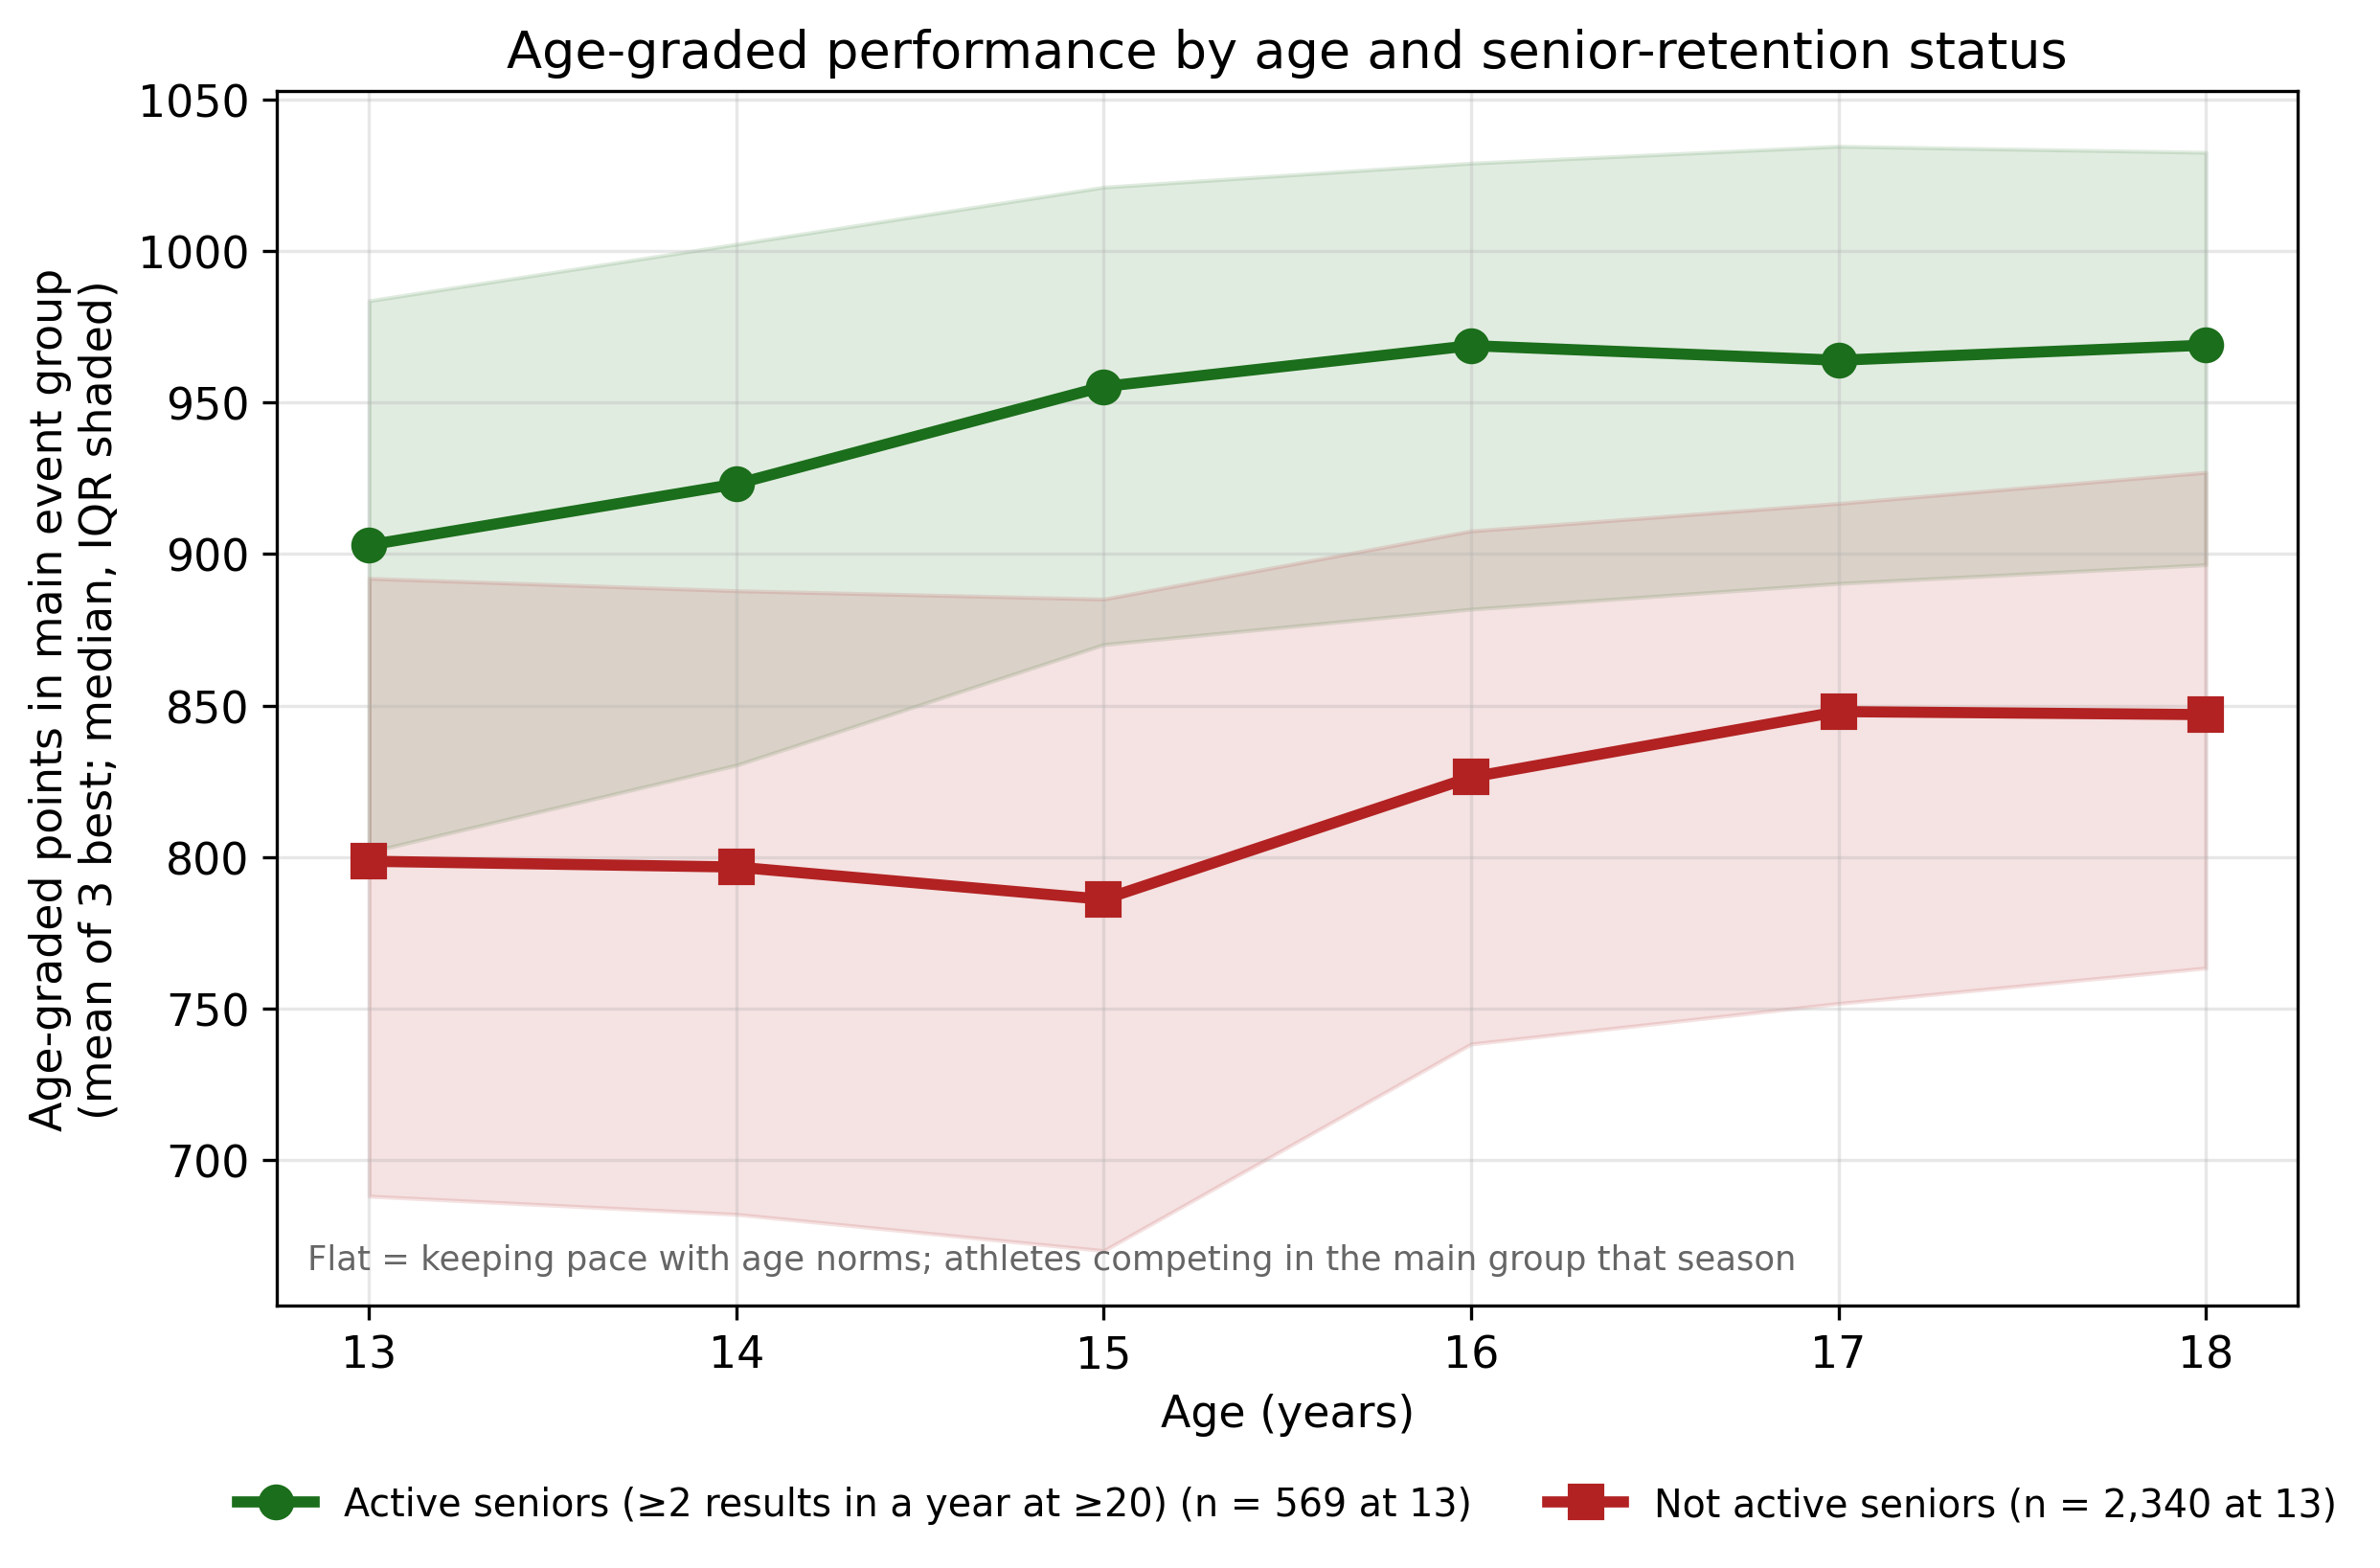
\includegraphics[width=0.95\textwidth]{fig1_performance_by_age.png}
\caption{Age-graded performance (mean of three best results in the main event group; median, IQR shaded) by age and senior-retention status, among athletes competing in the main group that season. Because the points are age-calibrated, a flat line means developing as the age norms expect. The late rise in the dropout group reflects progressive selection of the most persistent dropouts, not improvement of the group that started.}
\label{fig:age}
\end{figure}

\subsection{Progression predicts senior retention (H1)}

Table~\ref{tab:models} reports the nested models. Adding progression to the full baseline model gave OR = 2.02 per SD (95\,\% CI 1.73--2.37; $p < .001$). In the same model, competition volume at 15--16 remained the strongest predictor (OR 3.15 per SD, 95\,\% CI 2.54--3.92), volume at 13--14 added nothing given later volume (OR 0.95), and women were less likely to remain than men with the same level, volume, and progression (OR 0.59, 95\,\% CI 0.48--0.73). The coefficient on baseline level rose from 1.70 in M1 to 2.35 in M2, as the reparametrisation in Methods implies: once the change is held fixed, the baseline coefficient absorbs the full weight of the implied later level. Cross-validated discrimination rose from AUC 0.855 (M1) to 0.864 (M2), a gain of 0.009 (95\,\% interval 0.008--0.010), with good calibration (slope 0.97; Brier 0.098). The association is thus strong at the individual level while the incremental discrimination beyond an already rich behavioural model is modest.

Figure~\ref{fig:quintile} shows the gradient descriptively. Within the highest tertile of later competition volume ($\geq$19 competition days over ages 15--16), senior retention rose from 22.2\,\% in the lowest progression quintile to 49.7\,\% in the highest; within the middle tertile from 5.2\,\% to 14.7\,\%. In the lowest-volume tertile ($\leq$5 days) retention was 1.4--3.7\,\% in every quintile: where engagement had already collapsed, progression distinguished little. This volume dependence was not a pre-specified hypothesis and should be read as exploratory.

\begin{table}[H]
\centering
\caption{Nested logistic models for senior activity (age $\geq$20) in the primary sample (n = 3\,808; 648 events). OR (95\,\% CI) per SD unless noted.}
\label{tab:models}
\small
\begin{tabular}{lcc}
\toprule
Predictor & M1 & M2 \\
\midrule
Progression 13--14 $\to$ 15--16, per SD & --- & 2.02 (1.73--2.37) \\
Performance level 13--14, per SD & 1.70 (1.45--2.00) & 2.35 (1.97--2.81) \\
Competition days 13--14, per SD & 0.79 (0.59--1.06) & 0.95 (0.70--1.28) \\
Competition days 15--16, per SD & 3.86 (3.14--4.76) & 3.15 (2.54--3.92) \\
Scored results 13--14, per result & 1.00 (0.98--1.01) & 1.00 (0.98--1.01) \\
Scored results 15--16, per result & 1.00 (0.99--1.01) & 0.99 (0.98--1.00) \\
Female (vs.\ male) & 0.63 (0.51--0.77) & 0.59 (0.48--0.73) \\
\midrule
Cross-validated AUC & 0.855 & 0.864 \\
$\Delta$AUC M2 $-$ M1 (95\,\% interval) & \multicolumn{2}{c}{0.009 (0.008--0.010)} \\
Calibration slope / Brier (M2) & \multicolumn{2}{c}{0.97 / 0.098} \\
\bottomrule
\end{tabular}
\vspace{0.3em}
\parbox{0.92\textwidth}{\footnotesize Both models additionally adjust for birth cohort, region, and club size. Because progression is the difference between the 15--16 and 13--14 scores, M2 is a reparametrisation of a model with both period levels; the progression OR equals the contribution of the later level given the earlier one.}
\end{table}

\begin{figure}[H]
\centering
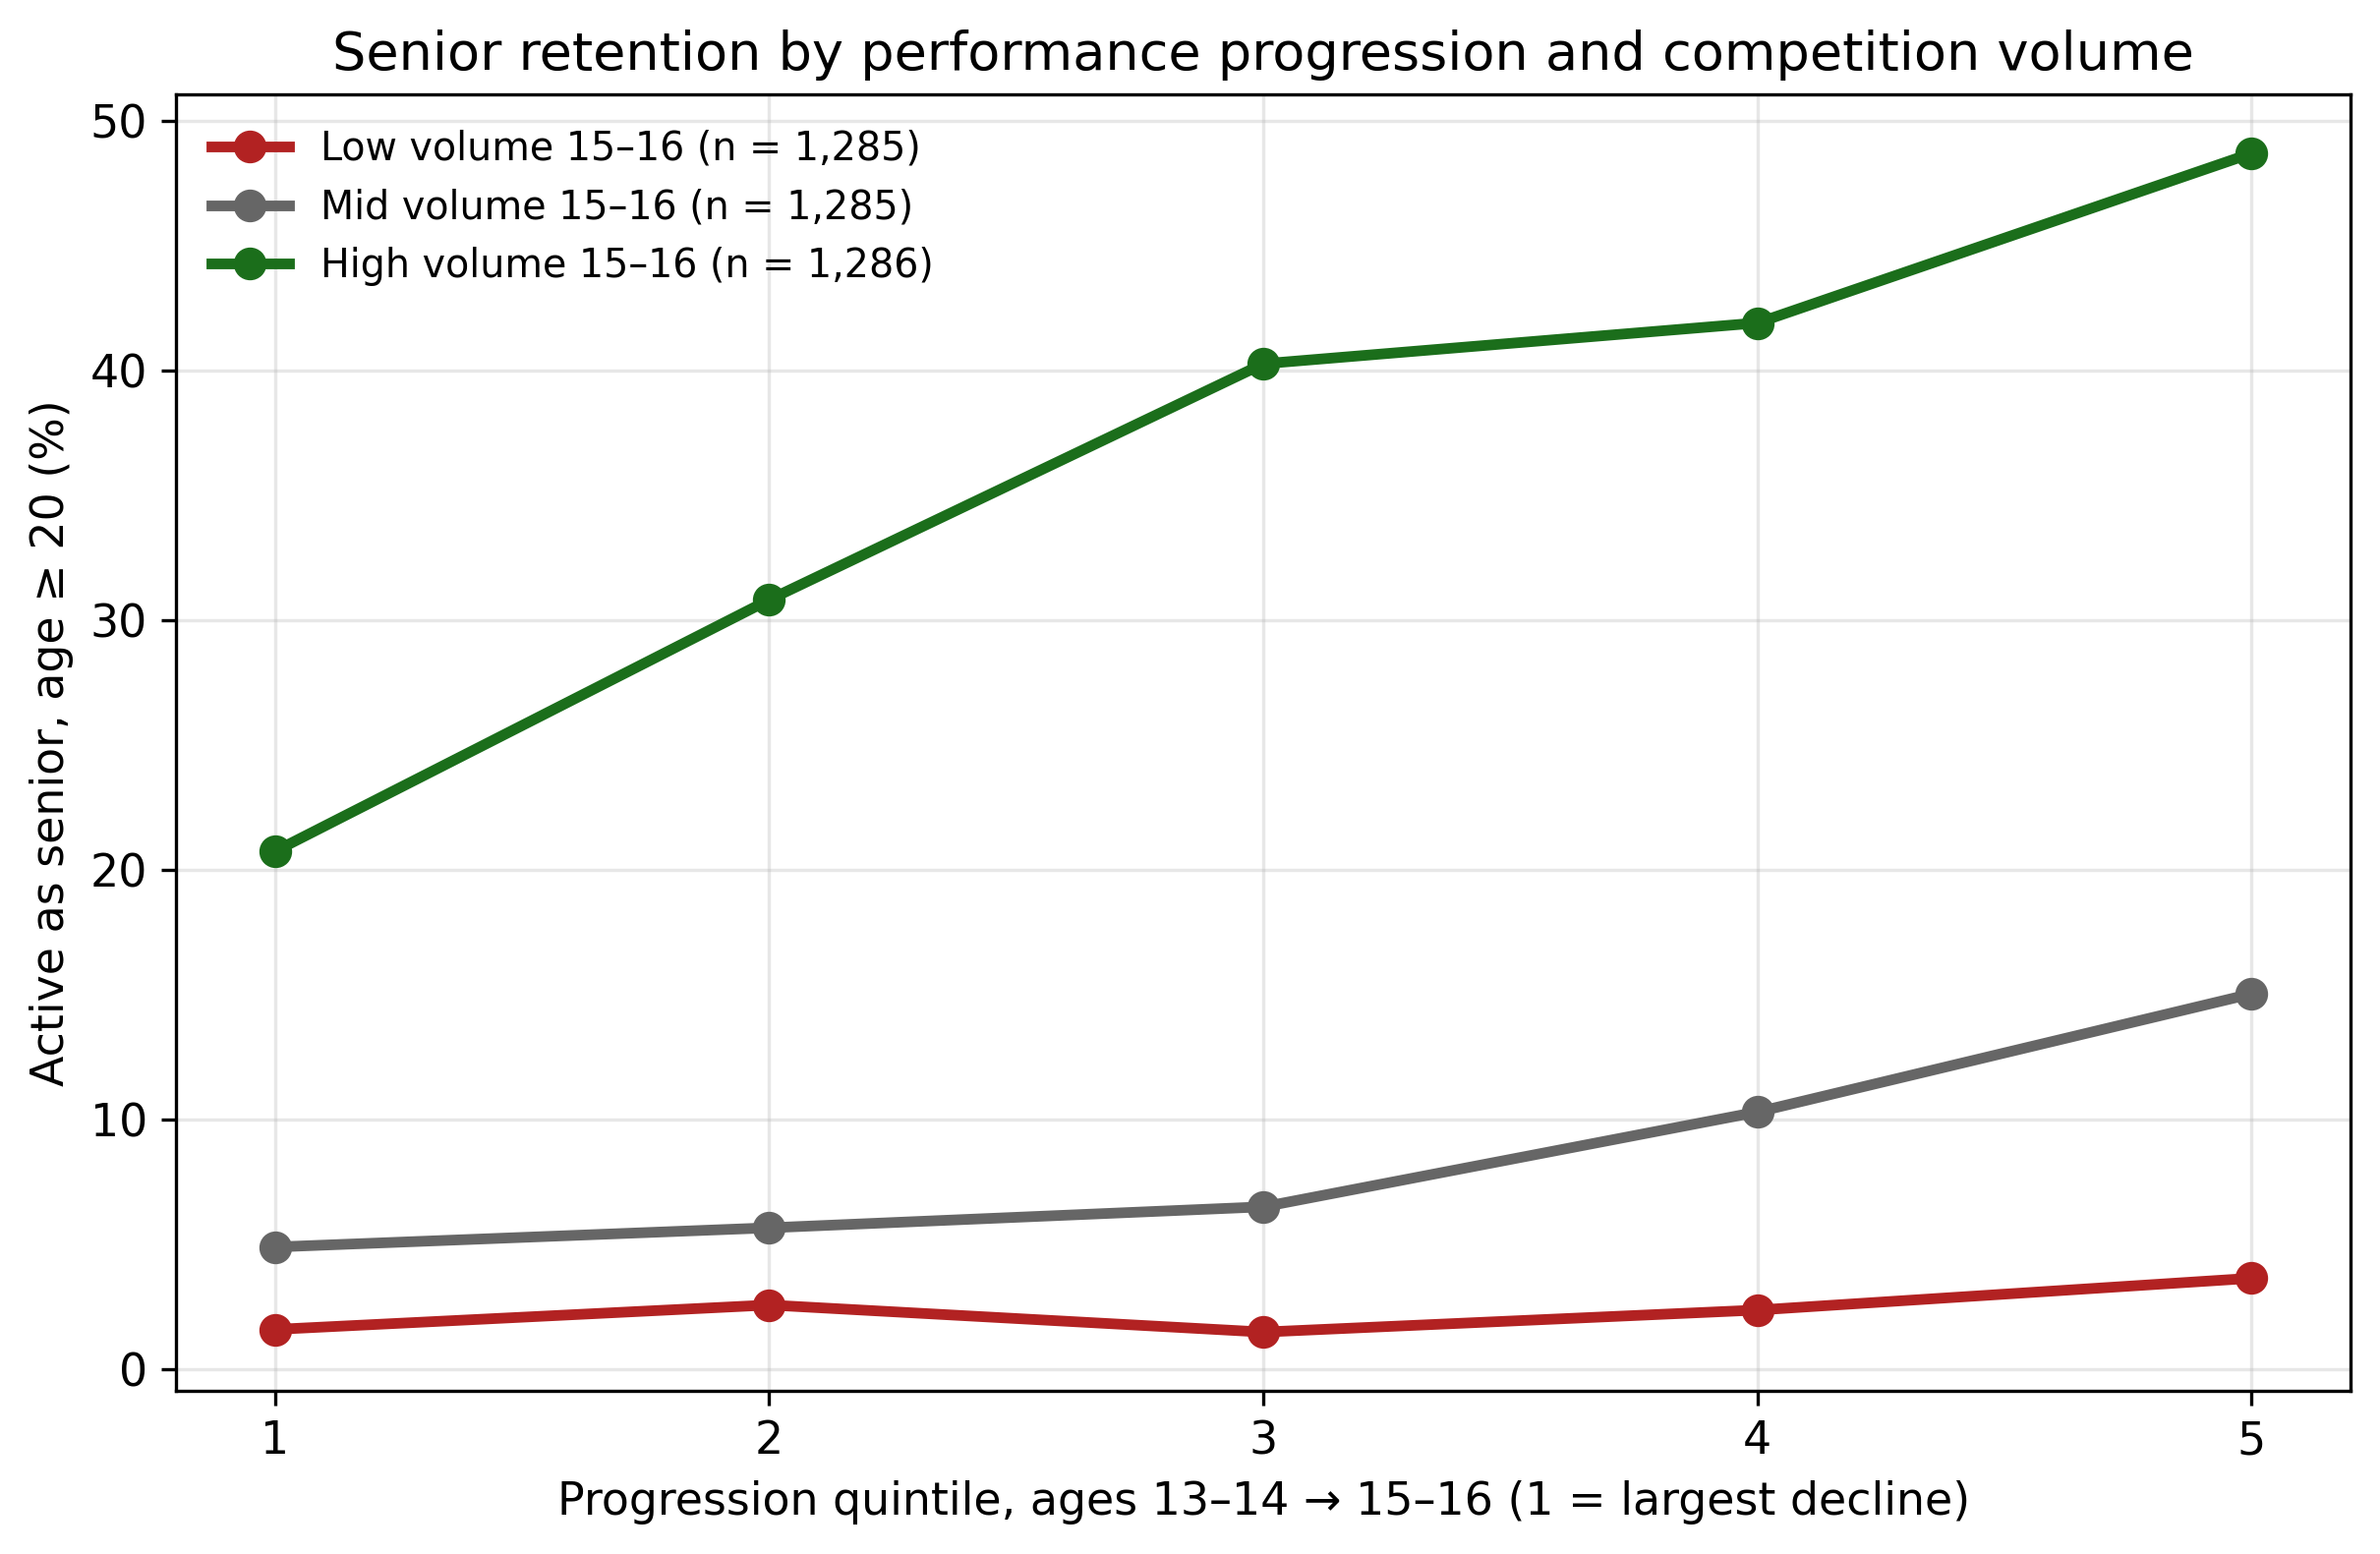
\includegraphics[width=0.85\textwidth]{fig3_retention_by_progression.png}
\caption{Senior retention by progression quintile within tertiles of competition volume at ages 15--16 (tertile bounds: $\leq$5, 5--19, $\geq$19 competition days across the two seasons). The progression gradient is concentrated where engagement is still present; this stratified display is exploratory.}
\label{fig:quintile}
\end{figure}

\subsection{No relative-age specificity (H2)}

The pre-specified test of the mastery-experience interpretation failed to find the predicted pattern (Table~\ref{tab:h2h3}). The progression $\times$ birth-quarter interaction was null (OR 0.95 per quarter, 95\,\% CI 0.85--1.07, $p$ = 0.40), with a point estimate in the \emph{opposite} direction of the prediction. Progression predicted retention in both halves of the birth year: OR 2.19 (1.76--2.72) among athletes born in Q1--Q2 and 1.89 (1.49--2.41) among those born in Q3--Q4.

\subsection{Progression versus level (H3)}

Given sex and competition volume, replacing performance level with progression left discrimination essentially unchanged: cross-validated AUC 0.854 with progression versus 0.855 with level (difference $-$0.001, 95\,\% interval $-$0.002 to $-$0.001). Progression does not discriminate \emph{better} than level; the two carry overlapping performance information, and the distinctive finding of H1 is that the change adds to the level, not that it replaces it.

\begin{table}[H]
\centering
\caption{Relative-age specificity (H2) and progression versus level (H3).}
\label{tab:h2h3}
\small
\begin{tabular}{lcc}
\toprule
Analysis & Estimate & $p$ \\
\midrule
Progression $\times$ birth-quarter trend (OR per quarter) & 0.952 (0.849--1.067) & 0.40 \\
Progression per SD, born Q1--Q2 & 2.19 (1.76--2.72) & $<$.001 \\
Progression per SD, born Q3--Q4 & 1.89 (1.49--2.41) & $<$.001 \\
\midrule
CV-AUC: sex + volume + progression & 0.854 (0.853--0.855) & \\
CV-AUC: sex + volume + level & 0.855 (0.854--0.856) & \\
Difference (progression $-$ level) & $-$0.001 ($-$0.002 to $-$0.001) & \\
\bottomrule
\end{tabular}
\end{table}

\subsection{The slide before exit}

Figure~\ref{fig:slide} aligns non-censored dropouts at their final active season (ages 16--19). Two seasons before exit, their age-graded performance still sat at their own reference level (median +3.7 points against the season three years before exit, 95\,\% CI $-$0.7 to +10.0; n = 1\,011 with complete four-season performance trajectories). In the penultimate season it fell 7.0 points below (CI $-$14.5 to $-$1.0), and in the final season 47.7 points below (CI $-$54.0 to $-$42.0), in parallel with the collapse in competition volume (median $-$2 days in the penultimate and $-$6 days in the final season; n = 1\,497). The final-season performance drop should be read with one mechanical caveat: athletes compete less in their last season, so the mean of the three best scores is computed from fewer attempts, which by itself depresses the measure. The cleaner signal is the penultimate-season decline, where volume had only begun to fall. Stagnation, like withdrawal, is visible before the athlete leaves.

\begin{figure}[H]
\centering
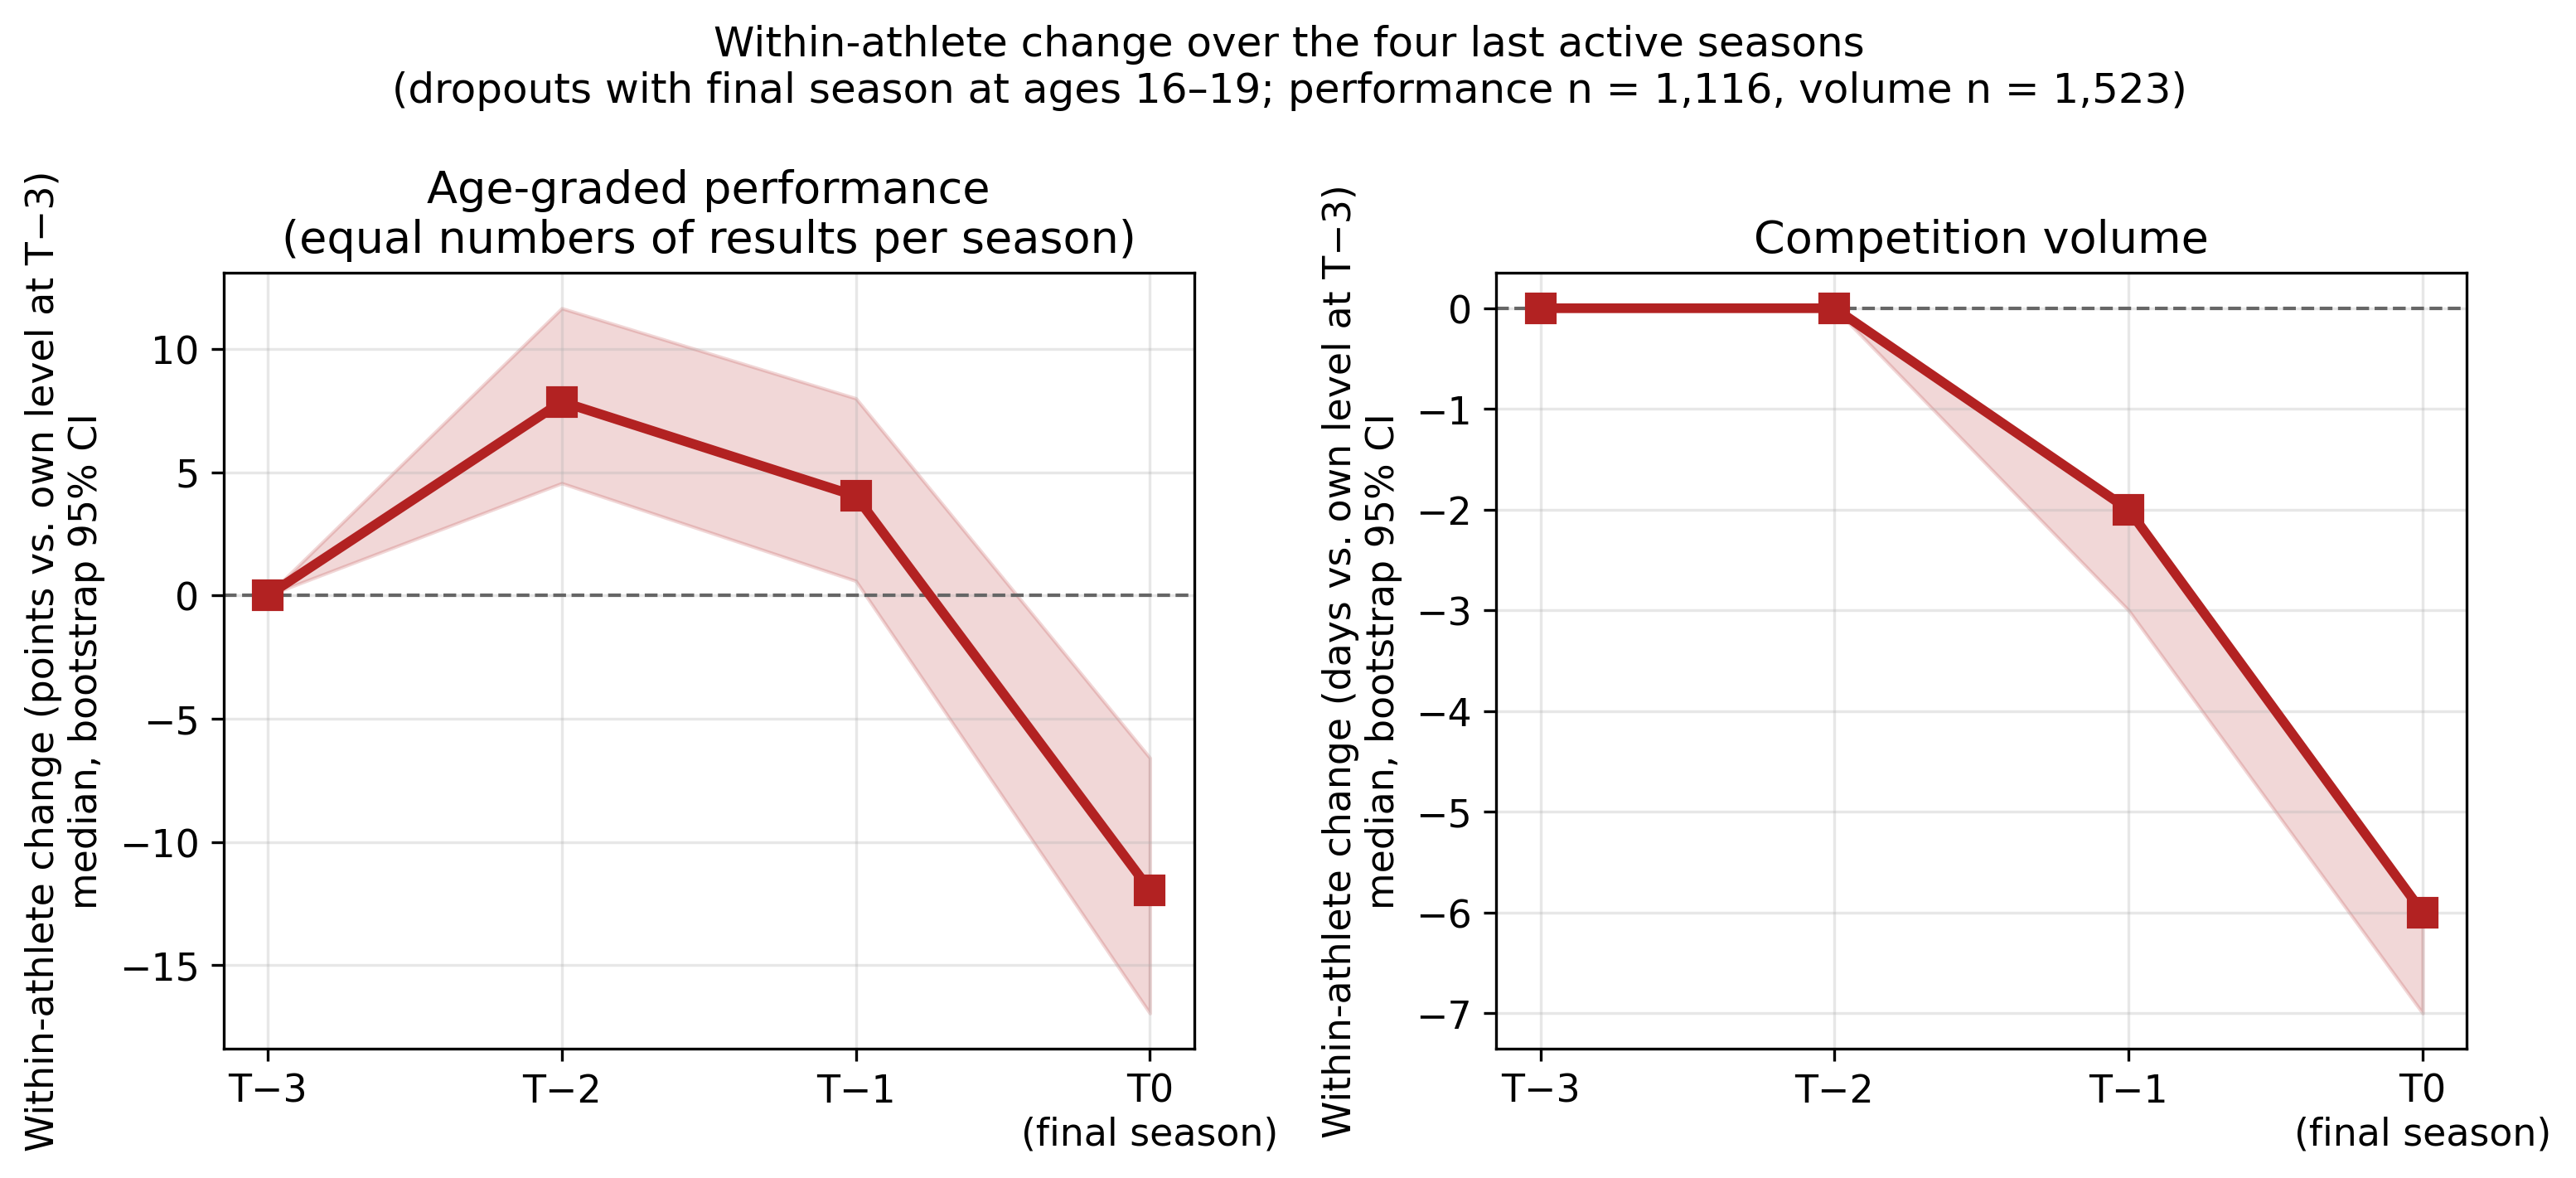
\includegraphics[width=\textwidth]{fig2_exit_aligned.png}
\caption{Within-athlete change over the four last active seasons among dropouts with a final season at ages 16--19 (medians with bootstrap 95\,\% CIs, relative to the athlete's own level three seasons before exit). Left: age-graded performance (points). Right: competition volume (days). The final-season performance drop is partly mechanical, as fewer competitions mean fewer attempts behind the mean-of-three-best score.}
\label{fig:slide}
\end{figure}

\subsection{Time-to-event and robustness}

In the landmark Cox model from age 17, progression was associated with a lower hazard of exit (HR 0.86 per SD, 95\,\% CI 0.83--0.90), alongside level (HR 0.82), dominant later volume (HR 0.47 per SD), null earlier volume given later (HR 1.01), and a higher hazard for women (HR 1.19, 95\,\% CI 1.11--1.28); Kaplan--Meier curves by progression tertile separated from the landmark onward (Figure~\ref{fig:km}). Table~\ref{tab:robust} collects the robustness analyses: the primary OR was stable across exposure definitions (season best 1.93; wind-legal marks 2.00; best event group at 15--16, which recovers event-group switchers, 1.92), strengthened when progression was measured from at least two results per window (2.18), held without the COVID-affected cohorts (1.95) with no clear COVID interaction (1.22, CI 0.91--1.63), held across outcome definitions (1.82--2.07; attenuated to 1.35 for the nearer outcome of activity at $\geq$18), replicated almost identically in the two cohort halves (2.00 and 2.03), and was unchanged under club-clustered inference. The within-baseline specification check was null (OR 1.00, 95\,\% CI 0.88--1.13), indicating that the cross-window estimate is not an artefact of result counts or of regression mechanics within a window. The E-value for the primary estimate was 2.84 (2.45 for the CI bound): an unmeasured confounder would need to roughly triple both the odds of high progression and of senior activity to explain the association away.

\begin{figure}[H]
\centering
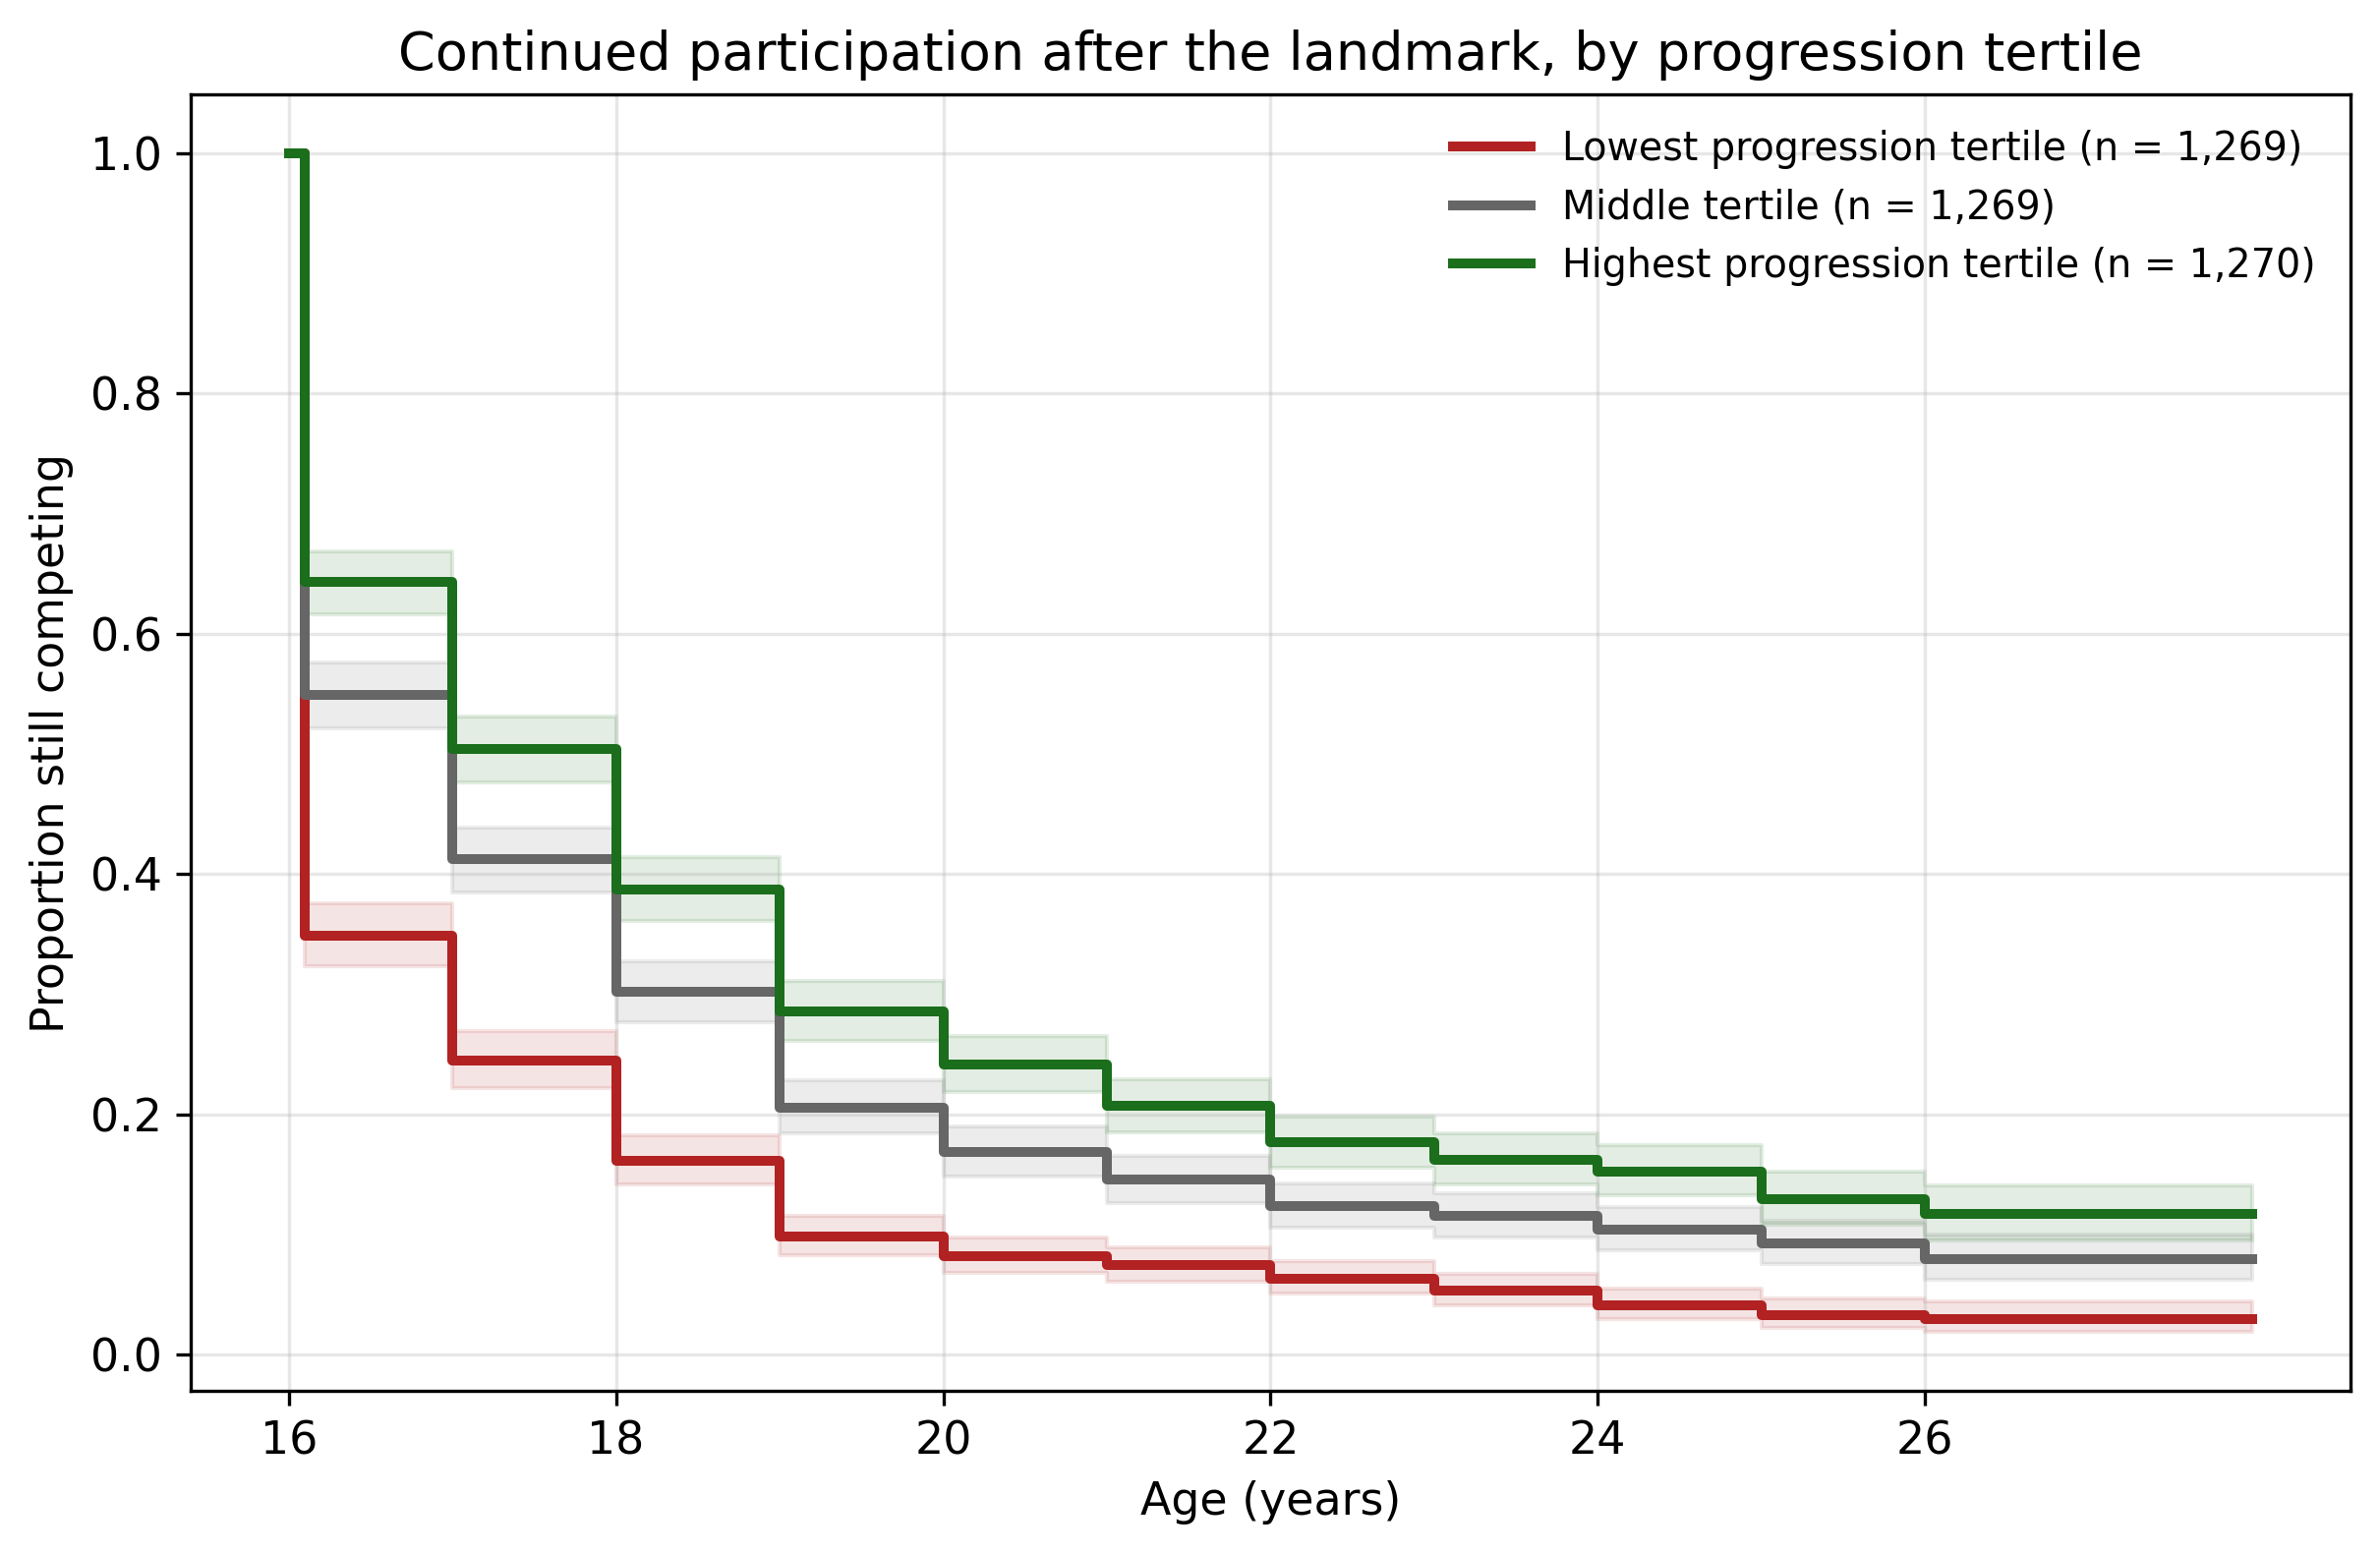
\includegraphics[width=0.85\textwidth]{fig4_km_progression.png}
\caption{Kaplan--Meier curves for continued participation after the landmark (age 16), by tertile of progression. Athletes active in 2025--2026 are censored.}
\label{fig:km}
\end{figure}

\begin{table}[H]
\centering
\caption{Robustness of the progression--retention association. OR (95\,\% CI) per SD of the exposure named; outcome is senior activity unless stated.}
\label{tab:robust}
\small
\begin{tabular}{lccc}
\toprule
Analysis & n & Events & OR (95\,\% CI) \\
\midrule
Primary: $\Delta$ mean of 3 best, main event group & 3\,808 & 648 & 2.02 (1.73--2.37) \\
Exposure: season best (maximum) & 3\,808 & 648 & 1.93 (1.66--2.25) \\
Exposure: mean of all results & 3\,808 & 648 & 1.59 (1.39--1.82) \\
Exposure: wind-legal marks only & 3\,761 & 646 & 2.00 (1.71--2.34) \\
Exposure: best event group at 15--16 (switchers included) & 3\,714 & 643 & 1.92 (1.67--2.22) \\
Specification check: $\Delta$ within ages 13$\to$14 & 2\,735 & 561 & 1.00 (0.88--1.13) \\
Excluding cohorts born 2004--2005 (COVID window) & 2\,894 & 498 & 1.95 (1.63--2.33) \\
Progression $\times$ COVID-window interaction & 3\,808 & 648 & 1.22 (0.91--1.63) \\
$\geq$2 scored results in both windows & 2\,997 & 625 & 2.18 (1.84--2.60) \\
Outcome: $\geq$1 result at age $\geq$20 & 3\,808 & 749 & 1.82 (1.58--2.09) \\
Outcome: $\geq$2 results in a year, ages 20--21 & 3\,808 & 612 & 2.07 (1.76--2.44) \\
Outcome: active at $\geq$18 (cohorts incl.\ 2006) & 4\,172 & 1\,640 & 1.35 (1.22--1.50) \\
Cohort A (born 1998--2001) & 1\,829 & 320 & 2.00 (1.60--2.51) \\
Cohort B (born 2002--2005) & 1\,979 & 328 & 2.03 (1.62--2.54) \\
Club-clustered robust SE & 3\,808 & 648 & 2.02 (1.70--2.41) \\
GEE, exchangeable club correlation & 3\,808 & 648 & 2.01 (1.70--2.38) \\
E-value for the primary OR (CI bound) & & & 2.84 (2.45) \\
\bottomrule
\end{tabular}
\end{table}

\FloatBarrier

% ════════════════════════════════════════════════════════════
\section{Discussion}

\subsection{Principal findings}

In the complete national registry population still competing at ages 15--16, an athlete's own performance progression over early adolescence predicted senior retention with an odds ratio of 2.0 per SD --- the same magnitude as competition volume, the strongest previously documented predictor in this system \cite{guttormsen2026dropout} --- independently of volume, baseline level, and the number of results, replicated across two birth cohorts, and robust to every pre-specified variation. Aligned at exit, dropouts' performance fell below their own earlier level in the penultimate season, before the final collapse of both performance and participation. Stagnation precedes exit. At the same time, two pre-specified results bound the finding: the association was no stronger among relatively younger athletes, and given volume, progression discriminated no better than level.

\subsection{Relation to the companion registry studies}

The result closes the gap the earlier registry studies left open between them. The development study showed that youth top lists turn over because athletes leave and are replaced, without following the leavers \cite{guttormsen2026development}; the cohort study showed that leavers withdraw behaviourally before they exit, without measuring their development \cite{guttormsen2026dropout}. The present study connects the two: the athletes who leave are, disproportionately, the athletes who had stopped progressing --- and their stagnation is visible in the registry before their departure, just as their declining participation is.

The reparametrisation noted in Methods gives the finding a second, equivalent reading. Because baseline level plus change is the same information as early level plus later level, H1 states that the \emph{later} performance level carries substantial information about retention beyond the earlier one. Current form, not early rank, is what the retention signal tracks. This mirrors, for performance, exactly what the companion study found for participation: there too, the later window dominated and the earlier one added nothing given it (both in the companion's volume models and in ours). The practical reading of both results is the same --- recent behaviour and recent development are what matter, which is also why the incremental \emph{discrimination} from adding progression to a model that already contains later volume is modest (+0.009 AUC). For prediction, participation remains the workhorse; progression tells the monitoring system \emph{why} an athlete's trajectory is bending, not only \emph{that} it is.

\subsection{What this means for the mastery interpretation}

The study was designed as the direct test the relative-age paper called for \cite{guttormsen2026rae}, and the outcome is split. The general premise of the mastery account --- that objective personal progress accompanies staying, independently of rank --- is strongly consistent with H1: progression predicts retention at every level of baseline performance, and the association survives adjustment for how often the athlete competes. But the account's distinctive prediction was specificity: personal progress should matter \emph{most} for relatively younger athletes, who lack rank-based reinforcement. That prediction failed. The interaction was null with a point estimate in the wrong direction, and progression predicted retention essentially equally in both halves of the birth year. Under our pre-stated interpretation rules, the registry evidence now favours a \emph{general} progression--retention link over a mastery mechanism specific to relative age. The relatively younger athletes' retention advantage documented in the companion cohort (OR 1.16 per quarter, conditional on volume and performance \cite{guttormsen2026dropout}) is, on this evidence, not explained by a heightened sensitivity to their own progress.

Three mechanisms, none separable in registry data, can produce the general link. Visible progress may sustain motivation (the mastery reading). Commitment may run the other way: athletes who have already decided to stay train more and therefore progress more, so that progression partly \emph{measures} commitment rather than causing it. And third causes --- injury above all --- can simultaneously halt development and drive exit; injury was the most common stated reason for dropout in the one long-term Norwegian athletics follow-up \cite{enoksen2011} and is invisible in competition records. The exit-aligned trajectories are equally consistent with all three. What the registry adds is not the mechanism but the observability: whichever process operates, it writes itself into ordinary competition records one to two seasons before the athlete disappears.

\subsection{The sex gap persists}

As in the companion cohort \cite{guttormsen2026dropout}, women left more often than men with the same volume, level, \emph{and now progression} (OR 0.59; Cox HR 1.19). The gap is not explained by women developing less: it is conditional on development. Its sources --- which may include competing time demands, environment, and body-related factors around puberty documented in the qualitative literature \cite{fraserthomas2008,crane2015} --- remain the most consequential unexplained pattern in this registry, and a study of its own.

\subsection{Practical implications}

Norwegian athletics already possesses, in its ordinary results database, both of the early-warning signals this research programme has now documented: declining participation \cite{guttormsen2026dropout} and, from this study, stagnating or declining age-graded performance among athletes who still compete. For a federation or club, the two signals answer different questions. Falling volume flags \emph{who} is disengaging; falling progression helps interpret \emph{why} a still-active athlete may be at risk, and identifies athletes whose exit the volume signal alone would catch only later. Given the modest incremental discrimination, we would not propose progression-based automated flags; the appropriate use is informal and conversational --- a coach noticing that an athlete has stopped improving against the age norms has, on this evidence, noticed something that doubles the odds of departure, whatever its cause. The exploratory volume dependence (Figure~\ref{fig:quintile}) suggests the conversation is most valuable while the athlete still competes regularly; once participation has collapsed, progression distinguishes little. Any operational use should respect the governance constraints discussed for behavioural monitoring in the companion paper (legal basis, designated recipients, opt-out) \cite{guttormsen2026dropout}, and none of this evidence supports using progression for talent \emph{selection} --- the companion development study shows precisely that early rankings mislead \cite{guttormsen2026development}.

\subsection{Strengths and limitations}

Strengths include complete national coverage of sanctioned competition from 2011, a landmark design that makes conditioning explicit, an exposure constructed to resist the mechanical maximum-of-$n$ bias and adjusted for result counts, internal replication across cohorts, a null within-baseline specification check, and sensitivity to clustering, COVID-19 exposure, and definitional choices.

The limitations are those of registry research, stated in advance. First, the estimates are associations; no causal effect of progression is claimed, and the three mechanisms above cannot be separated. Second, exit from the athletics registry is not exit from sport: transfer to other sports is invisible, which is why a null H1 would have been uninterpretable --- the asymmetry cuts the other way for the positive finding, since sport transfer would, if anything, generate athletes who leave \emph{while} progressing. Third, injury, training, and biological maturation are unobserved; maturation in particular could contribute to both slowed progression and exit in this age window. Fourth, the age-graded tables are unequally demanding across event groups; standardisation within sex and event group addresses comparisons, not the tables themselves. Fifth, the primary definition measures progression within the athlete's original main event group; athletes who changed groups entirely are excluded from the primary analysis, though the switcher-inclusive sensitivity gave the same answer. Sixth, results generalise to athletes still active at 15--16 in an open, club-based, low-cost competition system; absolute rates and thresholds will differ in gate-kept or pay-to-play systems. Finally, the study was not externally preregistered; the analysis plan, hypotheses, estimands, and interpretation rules were committed to version control before any exposure--outcome model was estimated, and all deviations would have been reported as such.

% ════════════════════════════════════════════════════════════
\section{Conclusions}

Among Norwegian youth track-and-field athletes still competing at ages 15--16, within-athlete performance progression predicted senior retention as strongly as competition volume does, independently of volume and level, and dropouts' stagnation was visible in the registry a season or more before they left. The association was general --- equally present among early- and late-born athletes --- supporting a broad link between visible development and continued participation, but not the relative-age-specific mastery mechanism proposed in earlier work on this registry. Competition records thus contain two complementary early signals of disengagement: athletes pull back, and they stop progressing, before they drop out. Understanding why --- commitment, injury, or motivation --- requires data the registry cannot provide, and is the natural next step.

% ── Declarations ────────────────────────────────────────────

\section*{Declarations}

\noindent\textbf{Funding.} The author received no funding for this work.

\medskip\noindent\textbf{Competing interests.} The author declares no competing interests. The author maintains an open, non-commercial statistics platform built on the federation's public results database.

\medskip\noindent\textbf{Ethics approval and consent.} The study analyses public competition results and falls outside the scope of the Norwegian Health Research Act; an assessment from Sikt was obtained. No individual athlete is identified. In accordance with the Norwegian children's sport regulations, no performance data below age 13 were analysed.

\medskip\noindent\textbf{Data availability.} The underlying data are the Norwegian Athletics Federation's public competition results. Aggregate outputs and all analysis code are available from the author; athlete-level analysis files are regenerable from the registry with the deposited code.

\medskip\noindent\textbf{Author contributions.} AGG conceived the study, performed all analyses, and wrote the manuscript.

\medskip\noindent\textbf{Declaration of AI use.} The author used a large language model (Claude, Anthropic) for programming assistance and manuscript drafting support. The author reviewed, verified, and edited all content and takes full responsibility for the integrity of the work.

\medskip\noindent\textbf{Acknowledgements.} The author thanks the Norwegian Athletics Federation, whose systematic registration of competition results over decades makes population research of this kind possible.

% ── References ──────────────────────────────────────────────

\bibliographystyle{unsrt}
\bibliography{references}

\end{document}
